\documentclass[tikz,border=5mm]{standalone}
\usepackage{tikz}
\usepackage{amsmath}

\usetikzlibrary{arrows.meta, positioning, calc}

\colorlet{colour_c}{gray!70!black}
\definecolor{colour_s}{HTML}{dfbb03}
\colorlet{colour_o}{red!90!black}

\begin{document}

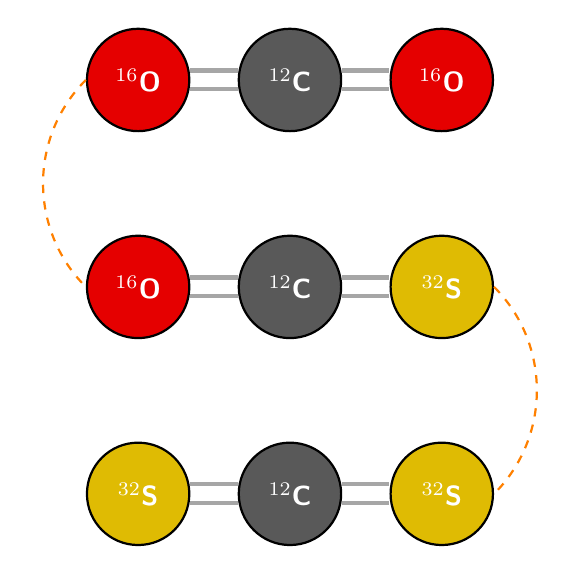
\begin{tikzpicture}
   [
      atom/.style={circle, draw, thick, minimum size=1.3cm, font=\sffamily\bfseries\color{white}},
      bond/.style={line width=1.5pt, gray!70},
      label node/.style={text=black, font=\sffamily\small},
   ]

   % =======================================================
   % Top Molecule: CO2
   % =======================================================

   % Atoms
   \node[atom, fill=colour_c] (C_CO2) {$^{12}\text{C}$};
   \node[atom, fill=colour_o, right=0.6cm of C_CO2] (Or_CO2) {$^{16}\text{O}$};
   \node[atom, fill=colour_o, left=0.6cm of C_CO2] (Ol_CO2) {$^{16}\text{O}$};

   % Double bonds
   \draw[bond] ($(C_CO2.east) + (0,0.12)$) -- ($(Or_CO2.west) + (0,0.12)$);
   \draw[bond] ($(C_CO2.east) - (0,0.12)$) -- ($(Or_CO2.west) - (0,0.12)$);

   \draw[bond] ($(C_CO2.west) + (0,0.12)$) -- ($(Ol_CO2.east) + (0,0.12)$);
   \draw[bond] ($(C_CO2.west) - (0,0.12)$) -- ($(Ol_CO2.east) - (0,0.12)$);

   % =======================================================
   % Middle Molecule: OCS
   % =======================================================

   % Atoms (below)
   \node[atom, fill=colour_o, below=1.3cm of Ol_CO2] (O_OCS) {$^{16}\text{O}$};
   \node[atom, fill=colour_c, below=1.3cm of C_CO2] (C_OCS) {$^{12}\text{C}$};
   \node[atom, fill=colour_s, below=1.3cm of Or_CO2] (S_OCS) {$^{32}\text{S}$};

   % Double bonds
   \draw[bond] ($(C_OCS.west) + (0,0.12)$) -- ($(O_OCS.east) + (0,0.12)$);
   \draw[bond] ($(C_OCS.west) - (0,0.12)$) -- ($(O_OCS.east) - (0,0.12)$);

   \draw[bond] ($(C_OCS.east) + (0,0.12)$) -- ($(S_OCS.west) + (0,0.12)$);
   \draw[bond] ($(C_OCS.east) - (0,0.12)$) -- ($(S_OCS.west) - (0,0.12)$);

   % =======================================================
   % Bottom Molecule: CS2
   % =======================================================

   % Atoms (below)
   \node[atom, fill=colour_s, below=1.3cm of O_OCS] (Sr_CS2) {$^{32}\text{S}$};
   \node[atom, fill=colour_c, below=1.3cm of C_OCS] (C_CS2) {$^{12}\text{C}$};
   \node[atom, fill=colour_s, below=1.3cm of S_OCS] (Sl_CS2) {$^{32}\text{S}$};

   % Triple bond (three parallel lines)
   \draw[bond] ($(C_CS2.west) + (0,0.12)$) -- ($(Sr_CS2.east) + (0,0.12)$);
   \draw[bond] ($(C_CS2.west) - (0,0.12)$) -- ($(Sr_CS2.east) - (0,0.12)$);

   \draw[bond] ($(C_CS2.east) + (0,0.12)$) -- ($(Sl_CS2.west) + (0,0.12)$);
   \draw[bond] ($(C_CS2.east) - (0,0.12)$) -- ($(Sl_CS2.west) - (0,0.12)$);

   % =======================================================
   % Arrows
   % =======================================================
    
   \draw[-, thick, orange, dashed] (Ol_CO2.west) to[out=225, in=135] (O_OCS.west);
   \draw[-, thick, orange, dashed] (S_OCS.east) to[out=-45, in=45] (Sl_CS2.east);

\end{tikzpicture}

\end{document}